\chapter{Problem Analysis}
%
The goal of this project is to develop a control strategy that can make an ASV suitable for survey tasks in water. More specifically, it should be able to perform bathymetric measurements.

In order to set up the requirements for the control system it is helpful to study a use case in which bathymetric measurements are already in use and where improvements in measurement techniques are needed.

The Port of Aalborg provides such a case along with previously used bathymetric measurements, see \autoref{fig:bathymetricMapPortOfAalborg}. These measurements are used by the Port of Aalborg to guide ships safely through the port without grounding.

\begin{figure}[H]
  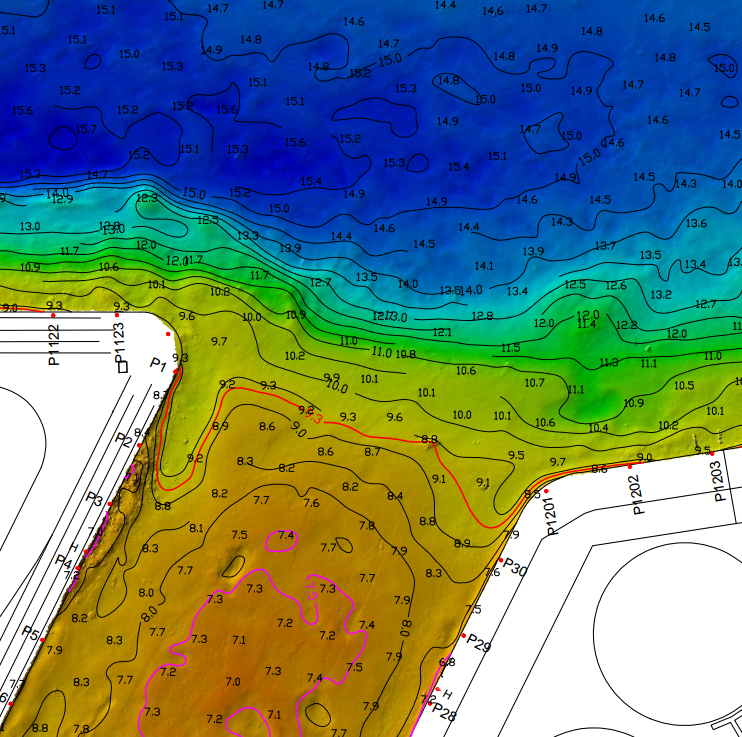
\includegraphics[width=0.5\textwidth]{figures/smallDebthMapAalborg}
  \caption{A cut from the full bathymetric map found in \autoref{app:bathymetricMapPortOfAalborg} provided by the Port of Aalborg.}
  \label{fig:bathymetricMapPortOfAalborg}
\end{figure}

The depths of the port are in constant change due to shifting sands. So while the bathymetric measurements help in guiding the ships by the safest route they are not currently provided frequently enough that this can be done in the most optimal manner. If two ships are heading towards each other, one of them is forced to wait in places where there is sure to be enough space for both in order to allow them to pass each other. However, this is sometimes an unnecessary precaution, if there was more recent knowledge of the depths in the port.

The measurements are currently performed by a manned vessel on which a multibeam echo sounder is installed. Contrary to single beam echo sounders, the multibeam can sweep a wider area. Nevertheless, this is still a time consuming task.

It is therefore desired to automate the process, preferably with a smaller unmanned vessel. This allows more frequent bathymetric measurements and improves the efficiency of guiding ships through the Port of Aalborg.

The vessel must be able to perform bathymetric measurements within an area autonomously. 
To do so it must be able to plan and follow a route, such that the entire area is measured. 
The route is dependent on the swath angle of the sensor and the precision of the controller. In order to ensure the entire area is covered, the path planner should include some overlap of the scanned areas, as this accounts for potential inaccuracies of the system.


%The controller design must be able to track references provided by a path planer as well as rejecting disturbances such as possible wind or the effect of the waves. This requires a model of the disturbances to be included in the controller design along with a robust controller capable of handling model uncertainties.

%The path planer must be able to design a route, in the form of waypoints\fxnote{not necessarily, is it not too early to decide?}, to reach all the positions needed to perform the different measurements required for the survey.

%The accuracy and precision with which the route can be tracked has a significant impact on the efficiency of the system. The less closely the path is tracked, the more overlap of the echo sounder beam is required from each sweep in order to cover the entirety of the bottom.

%The quality of the bathymetric measurements plays a part in determining the required overlap. Additionally other applications for the ASV would have requirements for the precision and accuracy provided by the control design. For these reasons and in order not to constrain the design to only one potential use, it is decided to set up some rather tight requirements for the system.


%From the project proposal it appears that a positioning accuracy of 0.1 m is desired. 
%From initial meetings with project supervisor, Jesper Abilgaard Larsen it was stated that a minimum precision of 0.3 m is required for the bathymetric measurements to be usable.\fxnote{Working on how to source this maybe use minutes?}

\section{Design Considerations}\label{sec:designconsiderations}
Following the S-44 IHO standards for hydrographic mapping, the measurements fall into the \emph{Special order} category, which sets a maximum total horizontal uncertainty (THU) of 2 m, 95\% confidence level for the position measurements. 
This standard is intended for under-keel measurements of the sea floor, which aligns with the scope of this project. \cite{IHO-S-44}

The Canadian Hydrography Service (CHS) includes a stricter category, the \emph{Exclusive order}. 
This category extends the \emph{Special order} category to be more focused on shallow waters, such as harbors. 
This category sets the maximum THU to be 30 cm with a 95\% confidence interval. 
It has been decided to use this standard as this is the one that best resembles the intended use case of the system. \cite{CHS}

The system design assumes that the sensor used to measure the depth of the Limfjord is based on the current multibeam echosounder used by the Port of Aalborg, the multibeam echosounder SeaBat 7125, which has a swath angle of 140$^\mathrm{o}$ \cite{echoSounder}.

Based on the bathymetric map found in \autoref{app:bathymetricMapPortOfAalborg}, a minimum depth is considered to estimate the width of the beam when it reaches the bottom. This width is used to plan the path that the boat needs to follow to reach all the points in a given area, see \autoref{chap:outerController}. In \autoref{fig:echosounder} a diagram of the echosounder's beam can be seen.

\begin{figure}[H]
    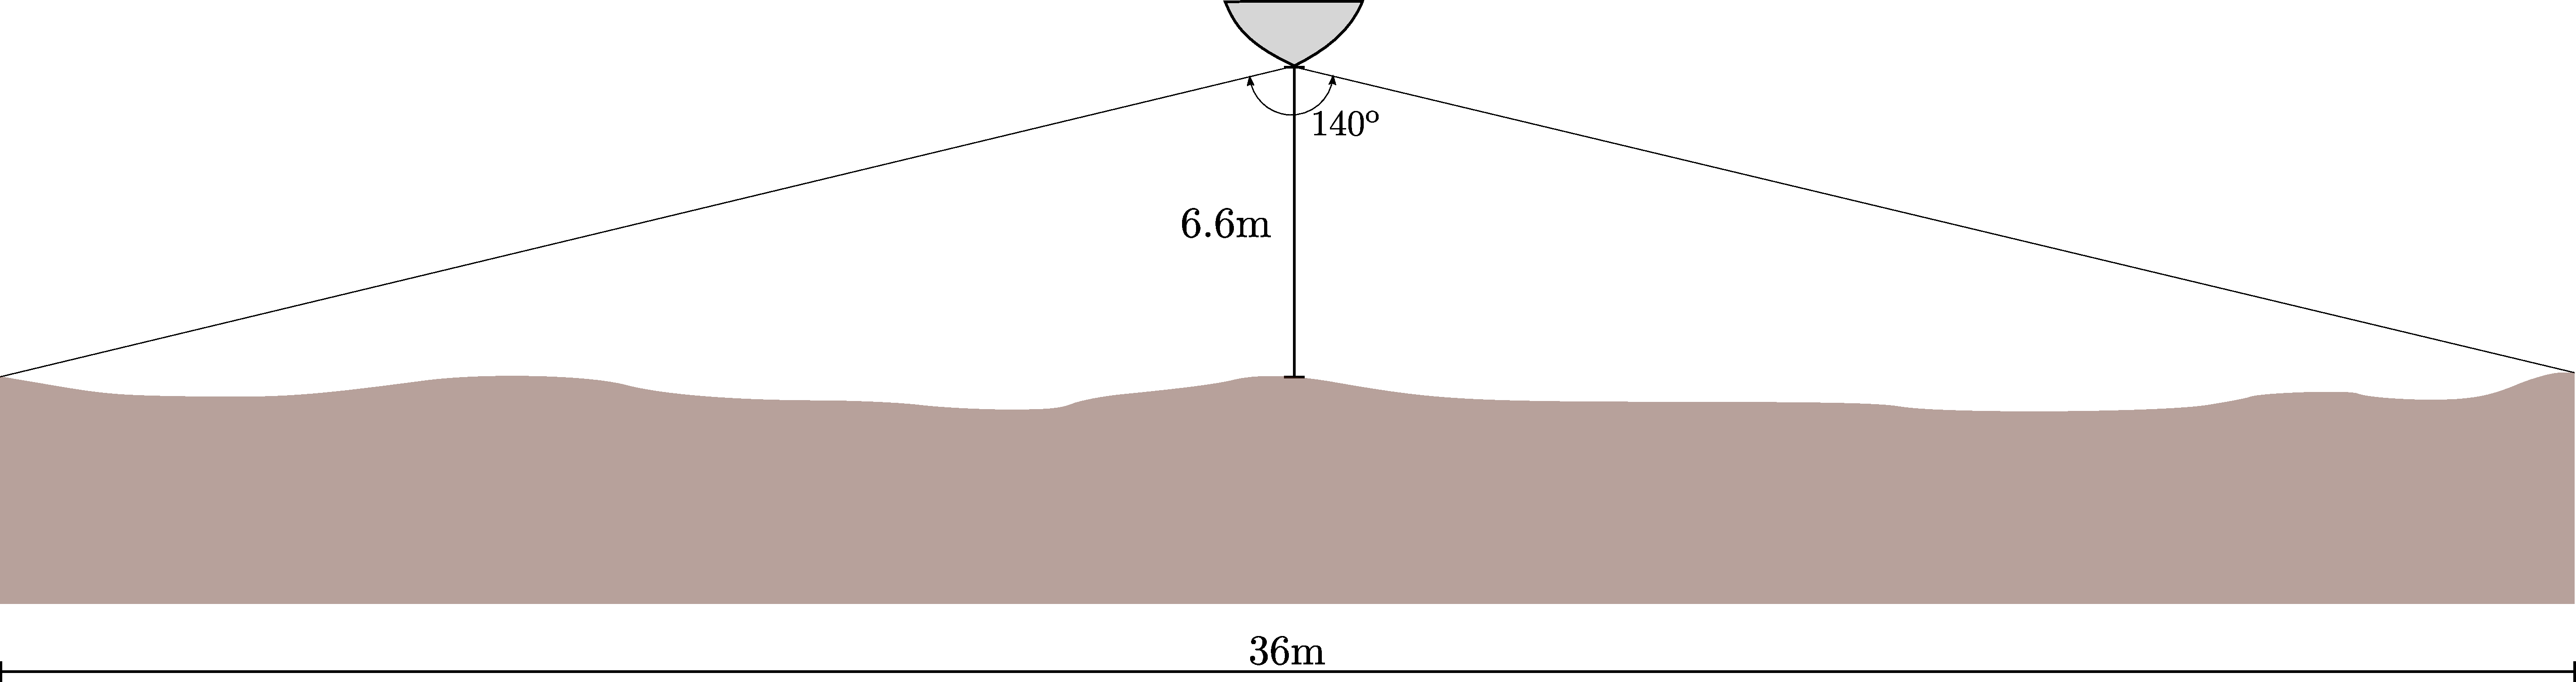
\includegraphics[width=0.9\textwidth]{figures/echosounder}
    \caption{Diagram of the echosounder's beam.}
    \label{fig:echosounder}
\end{figure}

%%%%%Communication%%%%%%%%%%%
As it is desired to have remote access to the vessel at all times, some form of communication between a operator and the vessel must be established. This is crucial for the implementation of safety features such as emergency stops, redirect the vessel or steer it back to land in case of system failures.

\section{Control Analysis}
For the vessel to autonomously survey an area, a control system is needed. 
The performance of the controller is crucial for how well the system performs overall. 
One of the challenges when designing a controller is how well it handles disturbances. 
In the case of the vessel the disturbances are mostly represented as wind, current and wave disturbances. 
\begin{figure}[H]
    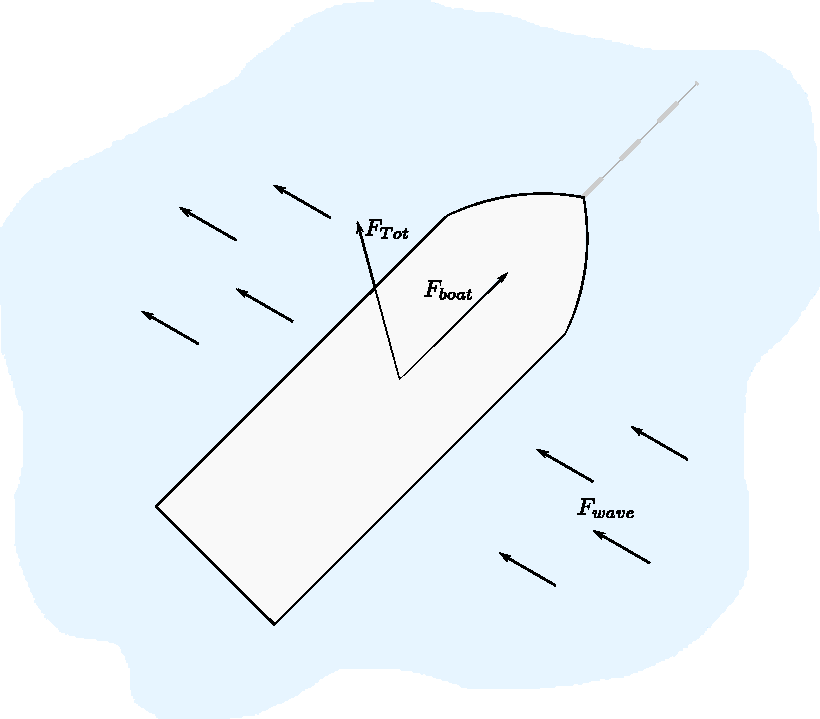
\includegraphics[width=0.5\textwidth]{figures/boatdisturbance}
    \caption{Illustration of how the vessel is affected by disturbances \fxnote{Should we mention the current}.}
    \label{fig:boatdist}
\end{figure}

As illustrated on \autoref{fig:boatdist}, these external forces alter the force vector of the vessel, influencing its trajectory. This results in a loss of operating range, as the vessel has to overlap a larger area to make sure the path covers the entirety of the survey area.

Additionally the controller could experience model inaccuracies. 
It is not possible to model a system perfectly, as it is always an approximation. 
These model variations influence the controller's performance and robustness as its design is based upon them. 

Another aspect of controller design is the energy consumption. The controller could be optimized such that it spends as little energy as possible reaching its destination. This feature gives the vessel a larger possible survey area as the ASV is a mobile platform and has a limited power supply. 

\section{Functional Requirements} \label{sec:requirements}
The design of a working prototype requires to set some functional requirements, and verify them once the design has been carried out.
%
\begin{itemize}
  \item[\textbf{A:}] It shall be possible to select the area in which the bathymetric measurements are to be performed.
  \item[\textbf{B:}] The ASV shall be able to plan a route, such that the entire survey area is mapped.
  \item[\textbf{C:}] The ASV shall be able to follow the planned route.
  \item[\textbf{D:}] The controller shall be robust to external disturbances.
  \item[\textbf{E:}] The THU shall not exceed 30 cm with a 95\% confidence interval.
  \item[\textbf{F:}] The ASV shall record and store data locally for extraction at the end of the survey.
  \item[\textbf{G:}] It shall be possible to give the ASV a command to stop and steer it back to land.
\end{itemize}
%
%The remainder of the problem analysis will go into how the functional requirements can be achieved. This will result in a set of technical requirements, which sets the perimeters of the design.






%\section{Technical Requirements}
%\fxnote{this section should be placed after analysis of sensors}
%Track position reference:\\
%- Summary of results of sensor capabilities\\
%- precision requirements for the control design\\
%- The bathymetry measurements are reliant on how much the boat tips, as it is single beam and measures shortest distance in the beam, some analysis must be done in this regard. Maybe it is necessary to stabilize the boat with floats on its sides. It would still be sensitive to waves, maybe the problem can be solved by measuring the tilt of the boat and mapping the measurements to the correct point in the inertial system having used beam and tilt angle to calculate vertical distance. This approach will put the measurements in a band around the path of the boat rather than in a straight line, question is if this is a good or a bad thing?
%
%Is it necessary to consider the water level on the day/time of the measurement? This is information which could be pulled from the Internet I think, either manually or, if the vessel has a connection, automatically.
%
%Record and store data:\\
%- Summary of results of data recordings (how much space is needed)\\
%- Space requirement for storing data\\
%- If chosen to send data back: requirement for communication\\
%
%Simple stop and call back commands:\\
%- communication requirement



